\section{Описание}
Прежде чем приступить к описанию реализованной структуры,  уместно рассказать о том классе деревьев, к которым она относится. Trie(название произошло от слова retireval)-деревья это структура данных, позволяющяя эффективно выполнять поиск, вставку и удаление в тех случаях, когда необходимо реализовать словарь, ключами в котором являются строки. Основная особенность таких деревьев заключается в хранении значений в нижней части дерева, то есть в листьях. В узлах, не являющихся листьями содержится набор символов алфавита, из которого состоят строки, и поставленных им в соответствие указателей на дочерние элементы. В алфавит необходимо добавить фиктивный символ, символизирующий окончание строки(и наличие её в данном дереве как ключа).  В итоге, поиск элемента в дереве сводится к последовательной проверке символов переданного ключа и к дальнейшему спуску по дереву на основании значения этого символа.\\

\begin{figure}[hb]
\center{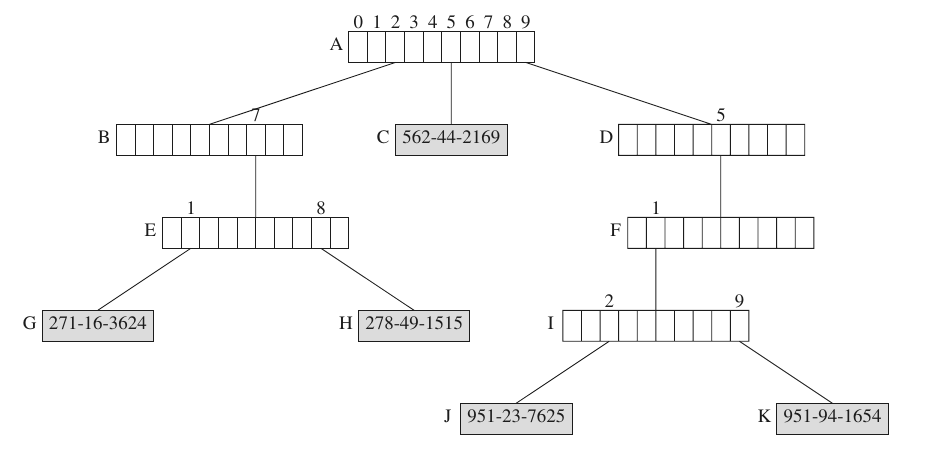
\includegraphics[scale=0.3]{trie.png}}
\caption{Пример trie}
\label{fig:image}
\end{figure}

Для trie, использующего битовое представление строк, Роберт Седжвик приводил такое определение.
\begin{displayquote}
Под trie-деревом понимается бинарное дерево, имеющее ключи, связанные с каждым из его листьев, и рекурсивно определённое следующим образом. Trie-дерево, состоящее из пустого набора ключей представляет собой нулевую связь. Trie-дерево, состоящее из единственного ключа --- это лист, содержащий данный ключ. И, наконец, trie-дерево, содержащее больше одного ключа --- это внутренний узел, левая связь которого ссылается на trie-дерево с ключами, начинающимися с 0 разряда, а правая --- на trie-дерево с ключами, начинающимися с 1 разряда, причем для конструирования поддеревьев ведущий разряд такого дерева должен быть удален.\cite{Sedgewick}
\end{displayquote}

Trie может быть преобразован в сжатый trie. Сжатие производится следующим образом: если начиная с узла X до некоторого его дочернего узла Y, каждый узел имеет лишь одного потомка, то все такие узлы можно убрать из дерева, добавив их ключи в узел X(теперь в нём хранится не один символ, а строка).\\

Вернёмся к структуре данных, которую нужно реализовать по условию лабораторной работы.
PATRICIA(Practical Algorithm To Retrieve Information Coded In Alphanumeric) --- особый сжатый бинарный trie, в каждом узле которого хранится ключ(строка, возможно в битовом представлении), значение, число, представляющее собой номер бита, значение которого будет проверяться при вставке или поиске, и две ссылки на некоторые элементы дерева. Для любого узла верно, что значение номер бита для проверки у его потомков строго больше, чем у самого узла(если это не так, значит ссылка на потомка на самом деле является ссылкой на элемент, находящийся выше по дереву, а в таком случае он не является потомком нашего узла, такая ссылка называется обратной). Стоит отметить, что любой элемент дерева, кроме корня(или header'а, как его ещё называют), имеет ровно две ссылки, в то время как корень имеет только левую ссылку.  Таким образом удаётся избегать однонаправленного ветвления. При вставке, удалении или поиске в одном узле необходимо сравнить всего один бит хранимого ключа и ключа, для которого совершается одно из трёх вышеприведённых действий. PATRICIA имеет сложность $O(h)$ для вставки, удаления и поиска, где $h$ --- высота дерева. Исходя из строения данной структуры, можно утверждать, что высота дерева не будет превышать битовой длины наибольшей из хранящихся в нем строк. Реализации алгоритмов вставки, удаления и.т.д. будут рассмотрены в следующем разделе.

\pagebreak

\section{Исходный код}

\subsection{Описание программы}
Программа предоставляет интерфейс для работы с вышеописанной структурой данных, принимая во входной поток строки с командами. Существует 5 возможных команд.
\begin{itemize}
  \item \textit{+ KEY VALUE} ---  Добавляет в дерево пару из ключа KEY и значения VALUE, если такого элемента ещё нет в дереве
  \item \textit{- KEY} --- Удаляет из дерева элемент с ключом KEY, если он существует
  \item \textit{KEY} --- Осуществляет поиск элемента с ключом KEY в дереве
  \item \textit{! Save PATH\_TO\_FILE} --- Сохраняет словаря в файл в компактном бинарном представлении
  \item \textit{! Load PATH\_TO\_FILE} --- Загружает словарь из бинарного файла, заменяя им текущий
\end{itemize}

Само дерево реализовано как шаблонный класс, шаблонным параметром является тип хранимого значения, строки при этом представлены в виде TVector<unsigned char>(TVector --- собственная реализация контейнера std::vector, которая применялась и в предыдущей лабораторной работе). Такое представление позволяет никоим образом не ограничивать длину строк, хранимых в дереве, и так же добавляет достаточно удобный интерфейс для работы со строками. Класс TPatricia имеет несколько публичных методов, позволяющих осуществлять вставку, удаление, поиск, сохранение в файл, загрузку из файла.\\
Рассмотрим реализации вышеописанных функций.
\subsubsection{Поиск} 
Пусть в дереве мы ищем элемент с ключом \textit{Key}. Начиная с корневого элемента дерева, будем спускаться по дереву. Проверим n-ный бит нашего ключа, где n --- номер бита для проверки, сохранённый в каждом узле дерева. если этот бит равен 0, нужно спуститься в левое поддерево и продолжить поиск, в ином случае, нужно продолжить спуск в правое поддерево. Когда ссылка по которой мы перешли окажется обратной, это значит, что мы нашли место, где может хранится элемент, который мы ищем. Осталось только сравнить ключ узла и \textit{Key}, если они совпадают, значит элемент найден. Нужно отметить, что в корне номер бита для проверки равен -1(при нумерации с нуля), так что из него нужно просто спуститься в левое поддерево.\\
\subsubsection{Вставка}
 Стратегия для вставки элемента в дерево такова:
\begin{itemize}
  \item Попытаться найти \textit{Key} в дереве. Пусть \textit{reachedKey} --- ключ в узле \textit{endNode}, где поиск элемента прекратился по причине перехода по обратной ссылке.
  \item Определить самую левую позицию \textit{lBitPos}, в которой \textit{Key} и \textit{reachedKey} различаются.
  \item Создать новый узел, при этом значения бита для проверки в этом узле должно быть \textit{lBitPos}, а ключ и значение соответственно равны ключу и значению элемента, который необходимо вставить. Вставить этот в некотором месте пути, который мы прошли при поиске ключа \textit{Key} таким образом, чтобы не нарушалось свойство возрастания битов для проверки при спуске по дереву. Такая вставка ломает ссылку из некоторого узла \textit{p} в \textit{q}. Теперь эта ссылка должна вести в созданный узел.
\item Если в \textit{Key} на позиции \textit{lBitPos} находится 1, то правая ссылка нового узла должна указывать на сам узел, а левая должна ссылаться на  \textit{q}. Если же на позиции \textit{lBitPos} находится 0, то наоборот.
\end{itemize}
\subsubsection{Удаление}
Для удаления существует всего 3 случая. \\
\begin{itemize}
  \item Если в дереве остался только корневой элемент и его нужно удалить, то дерево становится пустым.
  \item Если удаляемый элемент \textit{p} содержит ссылку на самого себя, нужно найти его родителя \textit{pParent}, а так же единственного потомка \textit{q}. Ссылку из \textit{pParent} в \textit{p} нужно заменить на ссылку в \textit{q}, а  \textit{p} просто удалить.
  \item Если удаляемый элемент \textit{p} не содержит ссылок на себя, необходимо найти несколько узлов дерева. Нам нужен элемент \textit{q}, содержащий обратную ссылку в \textit{p}, также нужно найти узел \textit{r}, содержащий обратную ссылку в \textit{q}. Так же необходимо найти  \textit{qParent} --- родителя \textit{q} и запомнить, в какое поддерево \textit{q} мы перешли при поиске узла \textit{r}. Далее необходимо поменять местами ключи и значения элементов \textit{p} и \textit{q}, ссылку из \textit{r} в \textit{q} заменить на ссылку в узел \textit{p}. Ссылку из \textit{qParent} в \textit{q} заменить на ссылку из \textit{qParent} в то поддерево \textit{q}, в которое мы переходили в процессе поиска узла \textit{r}. Теперь можно удалить узел \textit{q}.\cite{India}
\end{itemize} 
\subsubsection{Сохранение в файл}
Заведем в каждом узле дополнительное поле, которое будет уникальным идентификатором узла при сохранении в файл. Тогда, с помощью рекурсивного обхода в глубину можно пронумеровать вершины, заодно сохранив все вершины в TVector<Node*>. Далее, в файл записывается размер вектора узлов. После этого в файле сохраняется информация обо всех вершинах в следующем порядке: уникальный идентификатор, значение узла, размер ключа, ключ(строка), номер бита для проверки. Заметим, что если в дереве $n$ элементов, то ссылок в нем $2n-1$. Далее в файл записываются все ссылки дерева в формате: идентификатор узла, из которого выходит ссылка, идентификатор узла, в который идет ссылка, символ, сигнализирующий, левая или правая это ссылка.
\subsubsection{Считывание из файла}
Благодаря тем данным, которые мы сохранили в файл, из них можно быстро сконструировать дерево. Достаточно просто считать число элементов в дереве(\textit{b}), создать TVector<Node*> размера \textit{n}, заполнить данными и проставить ссылки. 

\pagebreak
\subsection{Таблица функций и методов}
\begin{longtable}{|p{7.5cm}|p{7.5cm}|}
\hline
\rowcolor{lightgray}
\multicolumn{2}{|c|} {TPatricia.h, вспомогательная функция}\\
\hline
bool getNthBit(const TVector<unsigned char>\& lhs, size\_t index)&Возвращает значения бита строки под номером index(если такого нет, возвращается false)\\
\hline
\rowcolor{lightgray}
\multicolumn{2}{|c|} {TPatricia.h, template<typename T> class TPatricia}\\
\hline
TPatricia() = default & Конструктор по умолчанию для дерева\\
\hline
$\sim$TPatricia() & Рекурсивный деструктор\\
\hline
TOptional<T> operator [] (const TVector<unsigned char>\& string) const & Ищет элемент в дереве по ключу\\
\hline
bool Insert(TVector<unsigned char> string, T data) & Добавляет элемент в дерево, возвращает false, если такой элемент в дереве есть\\
\hline
bool Insert(TVector<unsigned char> string, T data) & Добавляет элемент в дерево, возвращает false, если такой элемент в дереве есть\\
\hline
bool Erase(const TVector<unsigned char>\& string)&Удаляет элемент из дерева, если успешно удалено, возвращает true\\
\hline
void ScanFromFile(const char* filename)&Считывает дерево из файла и заменяет им текущее дерево\\
\hline
void PrintToFile(const char* filename) const&Записывает дерево в бинарном представлении в файл\\
\hline
void CountIds(Node* node, int\& id, TVector<Node*>\& nodes) const&Рекурсивно нумерует узлы уникальными идентификаторами, при этом записывая их в переданный вектор, помечена как константная потому, что не изменяет содержимое дерева, за исключением некоторых технических данных\\
\hline 
void DeleteTree(Node* node)&Рекурсивно удаляет дерево\\
\hline 
Node* SearchParentNode(Node* node) const&Находит родительский узел переданного узла\\
\hline 
Node* SearchKey(const TVector<unsigned char>\& string, Node** back = nullptr) const&Ищет узел по ключу. Возвращает узел, полученный после первого перехода по обратной ссылке при поиске, не гарантируя равенство переданного в функцию ключа и ключа в узле. Если задан параметр back, то после окончания работы функции в нем будет находится узел, имеющий обратную ссылку на найденный\\
\hline 
Node* SearchParentNode(Node* node) const&Находит родительский узел переданного узла\\
\hline
\hline
\rowcolor{lightgray}
\multicolumn{2}{|c|} {template<typename T> class TVector}\\
\hline
TVector() = default; & Конструктор без параметров\\
\hline
TVector(size\_t newSize) & Конструктор, принимающий размер нового вектора\\
\hline
TVector(size\_t newSize, T defaultVal) &Конструктор, принимающий размер и значение по умолчанию\\
\hline 
TVector(const TVector\& other)&Конструктор копирования, копирует значения из переданного вектора\\
\hline
TVector(TVector\&\& other)& Конструктор перемещения, перемещает в создаваемый объект указатель из other, в other указатель становится nullptr\\
\hline
~TVector() & Деструктор, освобождает выделенную память.\\
\hline 
T\& operator[] (size\_t index)& Оператор доступа по индексу, возвращает data[index].\\
\hline 
const T\& operator[] (size\_t index) const& Константная версия оператора доступа по индексу.\\
\hline
void PushBack(const T\& elem)&Добавляет elem в конец вектора, при необходимости совершая реаллокацию памяти\\
\hline 
T* begin()& Возвращает указатель на память, храняющуюся внутри вектора, название данной и трёх последующих функций не соответствует codestyle из-за того, что функции begin() и end() используются в range-based for.\\
\hline 
T* end()& Возвращает указатель на хранящуюся память, увеличенный на размер вектора.\\
\hline 
const T* begin() const& Константная версия метода begin().\\
\hline
const T* end() const& Константная верстия метода end().\\
\hline 
TVector\& operator=(const TVector\& other) & Копирующий оператор присваивания, возвращает ссылку на текущий объект.\\
\hline
TVector\& operator=(TVector\&\& other)& Перемещающий оператор присваивания, перемещает указатель на память из other, указатель в other становится nullptr. Возвращает ссылку на текущий объект.\\
\hline 
void ShrinkToFit()& Сжимает кусок памяти, которым владеет вектор до его реального размера.\\
\hline
size\_t Size() const & Возвращает размер вектора.\\
\hline
\hline
std::ostream\& operator << (std::ostream\& os, const TVector<T>\& vec)&Перегрузка оператора вывода для TVector\\
\hline
bool operator == (const TVector<T>\& lhs, const TVector<T>\& rhs)&Перегрузка оператора равенства для TVector\\
\hline
bool operator != (const TVector<T>\& lhs, const TVector<T>\& rhs)&Перегрузка оператора неравенства для TVector\\
\hline
\hline
\rowcolor{lightgray}
\multicolumn{2}{|c|} {TOptional.h, template<typename T> class TOptional}\\
\hline TOptional() = default & Конструктор по умолчанию\\
\hline explicit TOptional(const T\& newValue) & Конструктор от значения типа T\\
\hline const T\& operator* () const & Константный оператор разыменования\\
\hline T\& operator* () & Оператор разыменования\\
\hline operator bool() const & Оператор приведения к типу bool\\
\hline
\hline
\rowcolor{lightgray}
\multicolumn{2}{|c|} {main.cpp}\\
\hline TVector<unsigned char> strToVec(const char* str)&Трансформирует строку в TVector<unsigned char> \\
\hline int main() & Реализует интерфейс для доступа к дереву\\
\hline

\end{longtable}

\pagebreak

\section{Консоль}
\begin{alltt}
ilya@ilya-lenovo:~/CLionProjects/da_02/solution$ ls
main.cpp  Makefile  solution  TOptional.h  TPatricia.cpp  TPatricia.h  TVector.h
ilya@ilya-lenovo:~/CLionProjects/da_02/solution$ cat Makefile 
CXX = g++
CXXFLAGS = -std=c++11 -O2 -Wextra -Wall -Werror -Wno-sign-compare -Wno-unused-result -pedantic
FILES = main.cpp TPatricia.cpp
NAME = solution

all: example

example:
	$(CXX) $(CXXFLAGS) -o $(NAME) $(FILES)
clean:
	rm -f *.o $(NAME)
ilya@ilya-lenovo:~/CLionProjects/da_02/solution$ make
g++ -std=c++11 -O2 -Wextra -Wall -Werror -Wno-sign-compare -Wno-unused-result -pedantic -o solution main.cpp TPatricia.cpp
ilya@ilya-lenovo:~/CLionProjects/da_02/solution$ nano input 
ilya@ilya-lenovo:~/CLionProjects/da_02/solution$ cat input
+ a 10
a
+ abc 654
ABC
+ ttt 123
+ flgfk 677667
TtT
! Save file
- ttt
- flgfk
ttt
- abc
abc 
! Load file
abc
ttt
ilya@ilya-lenovo:~/CLionProjects/da_02/solution$ ./solution < input 
OK
OK: 10
OK
OK: 654
OK
OK
OK: 123
OK
OK
OK
NoSuchWord
OK
NoSuchWord
OK
OK: 654
OK: 123
ilya@ilya-lenovo:~/CLionProjects/da_02/solution$ hexdump file
0000000 0004 0000 0000 0000 0000 0000 0000 0000
0000010 000a 0000 0000 0000 0001 0000 0000 0000
0000020 ff61 ffff ffff ffff 01ff 0000 0000 0000
0000030 7b00 0000 0000 0000 0300 0000 0000 0000
0000040 7400 7474 0003 0000 0000 0000 0002 0000
0000050 0000 0000 5723 000a 0000 0000 0005 0000
0000060 0000 0000 6c66 6667 056b 0000 0000 0000
0000070 0300 0000 0000 0000 8e00 0002 0000 0000
0000080 0300 0000 0000 0000 6100 6362 0009 0000
0000090 0000 0000 0000 0000 0000 0000 0001 0000
00000a0 0000 0000 0130 0000 0000 0000 0100 0000
00000b0 0000 0000 3100 0001 0000 0000 0000 0002
00000c0 0000 0000 0000 0230 0000 0000 0000 0200
00000d0 0000 0000 0000 3100 0002 0000 0000 0000
00000e0 0003 0000 0000 0000 0330 0000 0000 0000
00000f0 0300 0000 0000 0000 3100 0003 0000 0000
0000100 0000 0000 0000 0000 0000 0030          
000010b

\end{alltt}
\pagebreak

